\section{Simulation study}
\label{sec:simulation}

\subsection{Design}
\label{sec:design}

\paragraph{Data.} Each data set has $n=300$ units, a covariate uniform on $[-3,3]$ and standard
normal errors. The eight designs are: D1, two crossing lines with equal weights and noise;
D2, three parallel lines three noise scales apart ($m=12$); D3, as D1 with weights $0.7$ and
$0.3$ ($m=10$); D4, as D1 with noise scales $0.5$ and $1.5$; D5, as D1 with high-leverage
outliers; D6, as D1 with uniform outliers; D7, as D1 with two further covariates of slope $1$
($m=12$); D8, two parallel lines six noise scales apart; $m=8$ unless stated. In D1, D3, D4
and D6 the two lines cross at the origin with slopes $\pm1.5$, so the groups overlap near the
crossing and even the Bayes classifier with known parameters labels about $9\%$ of the units
wrongly; an accuracy of about $0.91$ is the ceiling there, and essentially one in D8. Each
unit is replaced by an outlier independently with probability $\varepsilon$, so the realised
fraction of outliers varies around $\varepsilon$. Outliers in the response are shifted up or
down by a uniform amount between $15$ and $30$ times the average noise scale; high-leverage
outliers (D5) have their covariate redrawn uniformly on $[6,9]$, outside the design range, and
their response uniformly on $[-3,3]$; uniform outliers (D6) are spread over the bounding box
of the clean data enlarged by $20\%$, away from the true lines.

\paragraph{Competitors.} The main rival is TCLUST-REG \citep{garciaescudero2010robust}, from the
FSDA toolbox \citep{riani2012fsda}, run unmodified under GNU Octave with restriction factor $12$,
$1000$ random starts, $50$ refinement steps and no second-level trimming in the covariates, at
the two conservative levels $\alpha=0.25$ and $0.40$, followed by reweighting and then by the
recovery step. The reweighting attached to TCLUST-REG is our own rule, the map of
Section~\ref{sec:reweight} applied twice with $c=2.5$ and a median absolute deviation per group,
which carries the idea of \citet{dotto2018reweighting} to regression; it is not the incremental
scheme of that paper, which is examined separately (Supplement, Section~S6). ``TCLUST-REG,
reweighted'' denotes this construction throughout. The Supplement (Tables~S4 to~S11, S37
and~S38) holds the rows of a shorter search ($300$ starts, $10$ refinement steps,
$\alpha\in\{0.05,0.10,0.15,0.25,0.40\}$), which understated TCLUST-REG with three groups,
and those of the trimmed cluster-weighted model \citep{garciaescudero2017robust} and the
trimmed likelihood estimator \citep{neykov2007robust} at the same five levels. CTLE
\citep{chang2020componentwise} and the bisquare mixture of regressions \citep{bai2012robust}
were the competitors without a level from published software; they come from the R package
RobMixReg \citep{cao2026robmixreg}, as do the two trimmed methods. Four further competitors without a level were added after the first part had
been analysed: the mixture with Laplace errors of \citet{song2014robust}; the mixture of
contaminated normal regressions \citep{punzo2017robust,mazza2020mixtures}; a mixture with a
uniform noise component in the manner of \citet{banfield1993model}, the last two our
implementations; and sequential RANSAC \citep{fischler1981random}, which extracts the $K$
lines one at a time and is given the true noise scale, so it is an oracle benchmark, not a
competitor that can be run on data. Least squares with $50$ random starts is a reference
without protection (software and settings: Supplement, Section~S1). The monitoring approach
of \citet{torti2019assessing} leaves the choice of the level to the analyst; it enters the
comparison only through two automatic rules for reading a level off the monitoring path
(Section~\ref{sec:measures}).

\paragraph{Criteria.} Every method is given the true number of groups $K$ and returns $K$
coefficient vectors, from which every clean unit receives the label of its nearest fitted
line. The \emph{accuracy} is the fraction of clean units whose label agrees with the true one,
maximised over relabellings; trimmed and flagged units are treated alike, and a failed fit counts
as accuracy zero (failures were rare except for CTLE; Supplement, Section~S5). This labelling
ignores the estimated scales and weights, so it is not the Bayes rule of any method where the
groups differ in scale, as in D4, and it does not penalise trimming or flagging clean units as
such. The coefficient error, the flagged fraction and the computing time are therefore
reported as well (Section~\ref{sec:measures}), and so are the adjusted Rand index on all
units, with the outliers as a class of their own, and a misclassification rate that counts a
flagged clean unit as an error. By these two criteria the main pipelines rank as they do by accuracy: up to
$\varepsilon=0.20$ the mean adjusted Rand index is $0.719$ for ESF and $0.725$ and $0.715$ for
TCLUST-REG at levels $0.25$ and $0.40$ with reweighting and the recovery step, beyond it $0.660$
against $0.519$ and $0.714$ (Supplement, Table~S45). Labelling the clean units by TCLUST-REG's
own assignment instead of the nearest line changed its mean accuracy in D2, D4 and with four
groups by $-0.03$ to $+0.02$ (Supplement, Table~S49), so the criterion does not drive the
comparison.

\paragraph{Analysis plans.} The study was run in parts, and before each part a written plan
fixed the comparison to be made and its thresholds (Plans~1 to~5; Supplement, Table~S47, with
the digests of the plan files in Table~S34); the third part is descriptive. Four things
reported below were decided after all the plans: the main rival pipeline, TCLUST-REG with the
long search, reweighting and the recovery step; the three mixtures and sequential RANSAC; the
best-of-five rule of Section~\ref{sec:constants}; and a guard in the scoring scale of ESF for
groups fitted exactly (Section~\ref{sec:taxi}), which changed nothing on the $40$ simulated
data sets on which we checked it.

\subsection{Up to 20\% of outliers}
\label{sec:low}

Table~\ref{tab:mainlow} shows, for each design and method, the lowest mean accuracy over
$\varepsilon\in\{0,0.05,0.10,0.20\}$; if a method works only at the right trimming level, or
only with equal groups, at least one entry in its row is low. Supplement Table~S40 gives the
TCLUST-REG rows cell by cell, with the paired differences from ESF.

\begin{table}[!tb]
\centering
\footnotesize
\caption{Worst mean accuracy on clean units (the lowest of the cell means) with up to $20\%$ of outliers ($\varepsilon\in\{0,0.05,0.10,0.20\}$), by design. D1 to D8: first part ($50$ data sets per cell). $K=4$, small groups (80/20 and 85/15, including the fresh data of Plan~4), clustered outliers and other designs (sample size, moderate outliers, dependent covariates, $t_3$, skewed and heteroscedastic errors): third part and Plans~4 and~5. Column entries are minima over different sets of $\varepsilon$: D1 to D8 over the four values above, the other columns over the values of $\varepsilon\le0.20$ run in the third part and Plans~4 and~5. TCLUST-REG was run with $1000$ random starts and $50$ refinement steps (the rows with the level $0.30$ and with equal weights were run after the others); ``reweighted'' is our two-pass rule ($c=2.5$, median absolute deviation per group). Sequential RANSAC is given the true noise scale and is an oracle benchmark, not a competitor that can be run on data. CTLE and the mixtures were run with the starts of Supplement Section~S1. In D5, TCLUST-REG at level $0.25$ with $5\%$ second-level trimming in the covariates and reweighting ($300$ starts) reaches $0.86$ (Supplement, Table~S37). Values below $0.85$ in italics.}
\label{tab:mainlow}
\resizebox{\textwidth}{!}{%
\begin{tabular}{lcccccccccccc}
\toprule
Method & D1 & D2 & D3 & D4 & D6 & D7 & D8 & D5 & $K=4$ & Small & Clust. & Other \\
\midrule
ESF (with the recovery step) & 0.91 & 0.89 & 0.90 & 0.90 & 0.89 & 0.91 & 1.00 & 0.85 & 0.95 & \textit{0.83} & \textit{0.78} & 0.90 \\
ESF with $m=12$ in every design & 0.91 & 0.90 & 0.89 & 0.90 & 0.89 & 0.91 & 1.00 & 0.86 & 0.88 & \textit{0.83} & \textit{0.75} & 0.90 \\
ESF alone & 0.91 & 0.89 & 0.89 & 0.90 & 0.90 & 0.91 & 1.00 & 0.85 & 0.95 & \textit{0.60} & \textit{0.70} & 0.88 \\
\addlinespace
TCLUST-REG, $\alpha=0.25$, reweighted, then the recovery step & 0.91 & 0.89 & 0.91 & 0.90 & 0.91 & 0.91 & 1.00 & \textit{0.83} & 0.91 & 0.90 & 0.90 & 0.91 \\
TCLUST-REG, $\alpha=0.40$, reweighted, then the recovery step & 0.91 & \textit{0.83} & 0.91 & 0.90 & 0.91 & 0.91 & 1.00 & 0.87 & \textit{0.81} & 0.85 & 0.91 & 0.89 \\
TCLUST-REG, $\alpha=0.30$, reweighted, then the recovery step & 0.91 & 0.87 & 0.91 & 0.90 & 0.91 & 0.91 & 1.00 & 0.87 & 0.88 & 0.89 & 0.91 & 0.90 \\
TCLUST-REG, $\alpha=0.25$, equal weights, reweighted, then the recovery step & 0.91 & 0.90 & 0.91 & 0.90 & 0.91 & 0.91 & 1.00 & 0.86 & 0.96 & 0.89 & 0.90 & 0.90 \\
TCLUST-REG, $\alpha=0.25$, reweighted & 0.91 & 0.89 & 0.89 & 0.90 & 0.91 & 0.91 & 1.00 & \textit{0.83} & 0.91 & \textit{0.60} & 0.90 & 0.88 \\
TCLUST-REG, $\alpha=0.40$, reweighted & 0.91 & \textit{0.83} & \textit{0.66} & 0.90 & 0.91 & 0.91 & 1.00 & 0.87 & \textit{0.81} & \textit{0.56} & 0.91 & \textit{0.60} \\
\addlinespace
CTLE & 0.91 & \textit{0.59} & 0.87 & 0.85 & 0.87 & 0.89 & \textit{0.72} & \textit{0.73} & \textit{0.55} & \textit{0.64} & 0.86 & \textit{0.81} \\
Bisquare mixture & 0.89 & \textit{0.56} & 0.88 & 0.90 & 0.90 & 0.90 & \textit{0.80} & \textit{0.55} & \textit{0.47} & \textit{0.81} & \textit{0.57} & 0.85 \\
Laplace mixture & 0.91 & \textit{0.61} & 0.91 & 0.91 & 0.91 & 0.91 & 0.96 & \textit{0.58} & \textit{0.60} & 0.88 & \textit{0.63} & 0.90 \\
Contaminated normal mixture & 0.91 & \textit{0.52} & 0.91 & 0.91 & 0.91 & 0.91 & 1.00 & \textit{0.83} & \textit{0.65} & 0.91 & \textit{0.58} & 0.89 \\
Noise-component mixture & 0.91 & \textit{0.75} & 0.91 & 0.90 & 0.91 & 0.90 & \textit{0.81} & \textit{0.53} & \textit{0.65} & \textit{0.64} & \textit{0.61} & 0.88 \\
Sequential RANSAC (oracle: true noise scale given) & 0.91 & \textit{0.69} & 0.91 & 0.90 & 0.91 & 0.91 & 0.97 & \textit{0.54} & \textit{0.71} & 0.91 & \textit{0.84} & 0.90 \\
Least squares (50 starts) & \textit{0.53} & \textit{0.37} & \textit{0.70} & \textit{0.52} & \textit{0.58} & \textit{0.53} & \textit{0.53} & \textit{0.53} & \textit{0.49} & \textit{0.80} & \textit{0.61} & \textit{0.51} \\
\bottomrule
\end{tabular}}
\end{table}

The rows of TCLUST-REG show what a generous level costs and what the recovery step returns. At
level $0.40$ with reweighting, TCLUST-REG trims away the smaller group whenever the groups are
unequal: its worst accuracy is $0.66$ in D3, where the smaller group holds $30\%$ of the units,
and $0.56$ with groups of $15\%$ and $20\%$. The recovery step returns these groups ($0.91$ and
$0.85$) but does not repair three and four groups, where the level discards part of several
groups at once ($0.83$ and $0.81$ with or without the step). At level $0.25$ with reweighting
and the recovery step, TCLUST-REG is at $0.89$ or more in every design except D5 ($0.83$);
without the step it loses the small groups at $\varepsilon=0$ ($0.60$). TCLUST-REG was run
without second-level trimming in the covariates, so in D5 the high-leverage points can be
trimmed only through their residuals, hence the $0.83$; the adaptive form of that trimming did
not help either (Supplement, Section~S6.1).
ESF is at $0.85$ or more in every design except clustered outliers at $\varepsilon=0.20$
($0.78$) and groups of $80\%$ and $20\%$ with three covariates at $\varepsilon=0.20$ ($0.83$).
With four groups it reaches $0.95$, against $0.91$ for the level $0.25$ and $0.81$ for the level
$0.40$ with estimated weights, and is matched only by TCLUST-REG at level $0.25$ with equal
weights ($0.96$). CTLE and the four mixtures all fall below $0.85$ with three or four groups and with
high-leverage points. With three groups CTLE and the Laplace and bisquare mixtures are below least
squares with $50$ starts even without outliers ($0.78$, $0.66$ and $0.72$ against $0.90$), so
their default search is part of the failure; a start from least squares raised the two mixtures
we implemented to $0.89$ with three groups and $0.95$ with four without outliers, but not with
outliers, and $100$ starts did not help (Supplement, Tables~S21 and~S27). Sequential RANSAC, although given the true noise scale, falls to
$0.69$ with three parallel groups and $0.71$ with four.

\begin{table}[htbp]
\centering
\small
\caption{The choice of a trimming level: mean over cells of the mean accuracy on clean units, the
number of cells with a mean below $0.85$, and the worst cell, for all $123$ cells of the study
(Plans~1 to~5 and the third part; the $\varepsilon=0.30$ cells of the first part are excluded,
as the second part replaces them). ``Better'' and ``worse'' of the two levels are chosen in each
cell after the run, between TCLUST-REG at $0.25$ and at $0.40$, each with reweighting and the
recovery step. The last four rows were run after the others: the levels $0.30$ and $0.35$, and
the levels $0.25$ and $0.40$ with equal weights (option \texttt{equalweights} of FSDA), all with
the long search.}
\label{tab:level}
\resizebox{\textwidth}{!}{\begin{tabular}{lcccccc}
\toprule
 & \multicolumn{3}{c}{$\varepsilon\le0.20$ (89 cells)} & \multicolumn{3}{c}{$\varepsilon\ge0.25$ (34 cells)} \\
\cmidrule(lr){2-4}\cmidrule(lr){5-7}
Method & Mean & Below $0.85$ & Worst & Mean & Below $0.85$ & Worst \\
\midrule
ESF & 0.914 & 2 & 0.78 & 0.820 & 13 & 0.53 \\
ESF, $m=12$ in every design & 0.912 & 2 & 0.75 & 0.813 & 13 & 0.53 \\
TCLUST-REG, $\alpha=0.25$, rw, recovery & 0.917 & 1 & 0.83 & 0.693 & 26 & 0.51 \\
TCLUST-REG, $\alpha=0.40$, rw, recovery & 0.909 & 4 & 0.81 & 0.863 & 8 & 0.53 \\
Better of the two levels, chosen afterwards & 0.918 & 0 & 0.87 & 0.865 & 7 & 0.53 \\
Worse of the two levels & 0.908 & 5 & 0.81 & 0.691 & 27 & 0.51 \\
TCLUST-REG, $\alpha=0.25$, rw, no recovery & 0.890 & 11 & 0.60 & 0.695 & 26 & 0.51 \\
TCLUST-REG, $\alpha=0.40$, rw, no recovery & 0.827 & 31 & 0.56 & 0.869 & 7 & 0.54 \\
\addlinespace
TCLUST-REG, $\alpha=0.30$, rw, recovery & 0.915 & 0 & 0.87 & 0.794 & 17 & 0.53 \\
TCLUST-REG, $\alpha=0.35$, rw, recovery & 0.912 & 4 & 0.83 & 0.851 & 10 & 0.53 \\
TCLUST-REG, $\alpha=0.25$, equal weights, rw, recovery & 0.919 & 0 & 0.86 & 0.769 & 24 & 0.53 \\
TCLUST-REG, $\alpha=0.40$, equal weights, rw, recovery & 0.907 & 4 & 0.79 & 0.856 & 10 & 0.54 \\
\bottomrule
\end{tabular}}
\end{table}

Table~\ref{tab:level} sets the three pipelines against the choice an analyst has to make.
With up to $20\%$ of outliers, the better of the two levels, chosen after the run, never falls
below $0.85$, while the worse one does so in five cells. ESF, which chooses nothing, is within
$0.03$ of the better of the levels $0.25$ and $0.40$ in $83$ of the $89$ cells, above it by
more than $0.03$ in two (four groups at $\varepsilon=0.10$ and $0.20$) and below it by more
than $0.03$ in four: clustered
outliers and the three small-group designs of Plans~3 and~4 at $\varepsilon=0.20$, with gaps of
$0.03$ to $0.125$. Without the recovery step, the level $0.40$ falls below $0.85$ in $31$
cells, $27$ of them with unequal or small groups. These counts describe design points chosen
to probe weaknesses, not frequencies in any population of data sets. With $200$ data sets in
each of the eleven cells that decide the comparison ($150$ added; Supplement, Table~S50), the
standard errors of the paired differences fall to about $0.01$ and the conclusions stand: with
four groups ESF is ahead of TCLUST-REG at levels $0.25$ and $0.30$ by $0.03$ to $0.06$ and on a
par with the level $0.25$ with equal weights, and with a small group or clustered outliers at
$\varepsilon=0.20$ it is behind the level $0.25$ by $0.03$ to $0.09$.

The levels in between and equal weights trade one range of contamination for the other
(Table~\ref{tab:level}, last four rows). With reweighting and the recovery step, the level
$0.30$ falls below $0.85$ in no cell up to $20\%$ of outliers and in $17$ of the $34$ beyond,
the level $0.35$ in four and ten. Equal weights make the level $0.25$ the most accurate pipeline
up to $20\%$ (mean $0.919$, no cell below $0.85$; ESF is within $0.03$ of it in $85$ of the
$89$ cells and below it by more in four) but leave $24$ cells below $0.85$ beyond. They
change the summaries of the level $0.40$ little, although cell by cell they gain $0.01$ to
$0.05$ with three groups and $0.04$ to $0.05$ with four and lose up to $0.20$ with unequal or small groups. The two
pipelines that do best up to $20\%$ appear as rows of Table~\ref{tab:mainlow}: the level
$0.30$ has no entry below $0.85$ and reaches $0.88$ with four groups, where the level $0.25$
with equal weights reaches $0.96$ and ESF $0.95$. Over all $123$ cells the level $0.40$ with reweighting and the
recovery step has the highest mean ($0.897$), then the level $0.35$ ($0.895$), the level $0.40$
with equal weights ($0.893$) and ESF ($0.888$). By mean accuracy and by the number of cells within $0.03$ of ESF up to $20\%$, the level
$0.35$ is the closest to a level that serves both ranges: up to $20\%$ of outliers it is within $0.03$ of ESF in $83$ of the $89$ cells
(mean $0.912$ against $0.914$), ahead in two and behind in four, three of them with four groups,
where it loses $0.11$ to $0.13$; beyond $25\%$ it is ahead of ESF in $12$ of the $34$ cells and behind in four.
Table~\ref{tab:level} is descriptive: these levels were run after the analysis plans.

The criterion of Plan~1, in the seven designs without high-leverage points at
$\varepsilon\le0.20$, $28$ cells, was met in every cell by ESF alone, the largest shortfall
against the best competitor being $0.029$ (standard error $0.014$), and again by ESF with the
recovery step under Plan~3 (Supplement, Table~S1 and Section~S6). Its second criterion, that every
fixed-level competitor trail ESF alone by at least $0.05$ in some cell, was not met: TCLUST-REG at level
$0.25$ with reweighting was never more than $0.033$ below it, so this competitor was tested
again, on new data, at higher contamination.

\subsection{Beyond 25\% of outliers}
\label{sec:high}

Plan~2 asked whether TCLUST-REG at level $0.25$ with reweighting fails once the contamination
exceeds its level while ESF alone does not. The answer was yes, by a wide margin and by construction:
at $\varepsilon=0.30$ and $0.35$ this competitor fell to accuracies between $0.53$ and $0.62$
in D1, D4, D7 and D8, with the short search and with the long one (Table~\ref{tab:mainhigh}),
where ESF alone stayed above $0.87$.

\begin{table}[!tb]
\centering
\footnotesize
\caption{Worst mean accuracy on clean units with $25\%$ to $35\%$ of outliers. D1 to D8: second part, new data ($100$ data sets per cell); the other columns: third part at $\varepsilon=0.30$ only ($50$ data sets per cell), so column entries are minima over different sets of $\varepsilon$. Rows and conventions as in Table~\ref{tab:mainlow}. Values below $0.85$ in italics.}
\label{tab:mainhigh}
\resizebox{\textwidth}{!}{%
\begin{tabular}{lcccccccccccc}
\toprule
Method & D1 & D2 & D3 & D4 & D6 & D7 & D8 & D5 & $K=4$ & Small & Clust. & Other \\
\midrule
ESF (with the recovery step) & 0.91 & \textit{0.55} & \textit{0.84} & 0.90 & \textit{0.58} & 0.88 & 1.00 & \textit{0.53} & \textit{0.72} & \textit{0.75} & \textit{0.55} & 0.87 \\
ESF with $m=12$ in every design & 0.91 & \textit{0.56} & \textit{0.83} & 0.89 & \textit{0.55} & 0.87 & 0.98 & \textit{0.53} & \textit{0.77} & \textit{0.66} & \textit{0.56} & 0.87 \\
ESF alone & 0.91 & \textit{0.56} & \textit{0.84} & 0.90 & \textit{0.59} & 0.88 & 1.00 & \textit{0.53} & \textit{0.73} & \textit{0.73} & \textit{0.54} & 0.87 \\
\addlinespace
TCLUST-REG, $\alpha=0.25$, reweighted, then the recovery step & \textit{0.53} & \textit{0.51} & \textit{0.70} & \textit{0.53} & \textit{0.69} & \textit{0.53} & \textit{0.53} & \textit{0.53} & \textit{0.74} & \textit{0.82} & \textit{0.59} & \textit{0.52} \\
TCLUST-REG, $\alpha=0.40$, reweighted, then the recovery step & 0.91 & \textit{0.76} & 0.87 & 0.90 & \textit{0.72} & 0.90 & 1.00 & \textit{0.53} & \textit{0.76} & \textit{0.82} & \textit{0.70} & 0.91 \\
TCLUST-REG, $\alpha=0.30$, reweighted, then the recovery step & \textit{0.60} & \textit{0.61} & \textit{0.74} & \textit{0.63} & \textit{0.73} & \textit{0.59} & \textit{0.60} & \textit{0.53} & \textit{0.77} & 0.86 & \textit{0.62} & \textit{0.77} \\
TCLUST-REG, $\alpha=0.25$, equal weights, reweighted, then the recovery step & \textit{0.59} & \textit{0.66} & \textit{0.71} & \textit{0.57} & \textit{0.74} & \textit{0.57} & \textit{0.64} & \textit{0.53} & \textit{0.78} & \textit{0.82} & \textit{0.61} & \textit{0.75} \\
TCLUST-REG, $\alpha=0.25$, reweighted & \textit{0.53} & \textit{0.51} & \textit{0.70} & \textit{0.53} & \textit{0.78} & \textit{0.53} & \textit{0.53} & \textit{0.53} & \textit{0.74} & \textit{0.82} & \textit{0.55} & \textit{0.52} \\
TCLUST-REG, $\alpha=0.40$, reweighted & 0.91 & \textit{0.76} & 0.87 & 0.90 & 0.90 & 0.90 & 1.00 & \textit{0.54} & \textit{0.76} & \textit{0.81} & \textit{0.68} & 0.91 \\
\addlinespace
CTLE & \textit{0.65} & \textit{0.40} & \textit{0.65} & \textit{0.47} & \textit{0.67} & \textit{0.55} & \textit{0.66} & \textit{0.51} & \textit{0.47} & \textit{0.62} & \textit{0.67} & \textit{0.69} \\
Bisquare mixture & \textit{0.73} & \textit{0.42} & \textit{0.82} & \textit{0.76} & \textit{0.83} & \textit{0.63} & \textit{0.75} & \textit{0.53} & \textit{0.46} & \textit{0.80} & \textit{0.57} & \textit{0.68} \\
Laplace mixture & 0.91 & \textit{0.48} & 0.90 & 0.91 & 0.90 & 0.90 & 0.94 & \textit{0.53} & \textit{0.53} & 0.86 & \textit{0.61} & 0.90 \\
Contaminated normal mixture & 0.90 & \textit{0.37} & 0.91 & 0.90 & \textit{0.67} & \textit{0.65} & 0.85 & \textit{0.61} & \textit{0.48} & 0.88 & \textit{0.53} & \textit{0.71} \\
Noise-component mixture & \textit{0.55} & \textit{0.40} & \textit{0.72} & \textit{0.55} & 0.87 & \textit{0.54} & \textit{0.53} & \textit{0.52} & \textit{0.46} & \textit{0.83} & \textit{0.57} & \textit{0.56} \\
Sequential RANSAC (oracle: true noise scale given) & 0.91 & \textit{0.64} & 0.91 & 0.91 & \textit{0.73} & 0.91 & 0.98 & \textit{0.53} & \textit{0.71} & 0.89 & \textit{0.63} & 0.90 \\
Least squares (50 starts) & \textit{0.53} & \textit{0.37} & \textit{0.70} & \textit{0.53} & \textit{0.53} & \textit{0.53} & \textit{0.53} & \textit{0.53} & \textit{0.47} & \textit{0.81} & \textit{0.62} & \textit{0.51} \\
\bottomrule
\end{tabular}}
\end{table}

\begin{figure}[tbp]
\centering
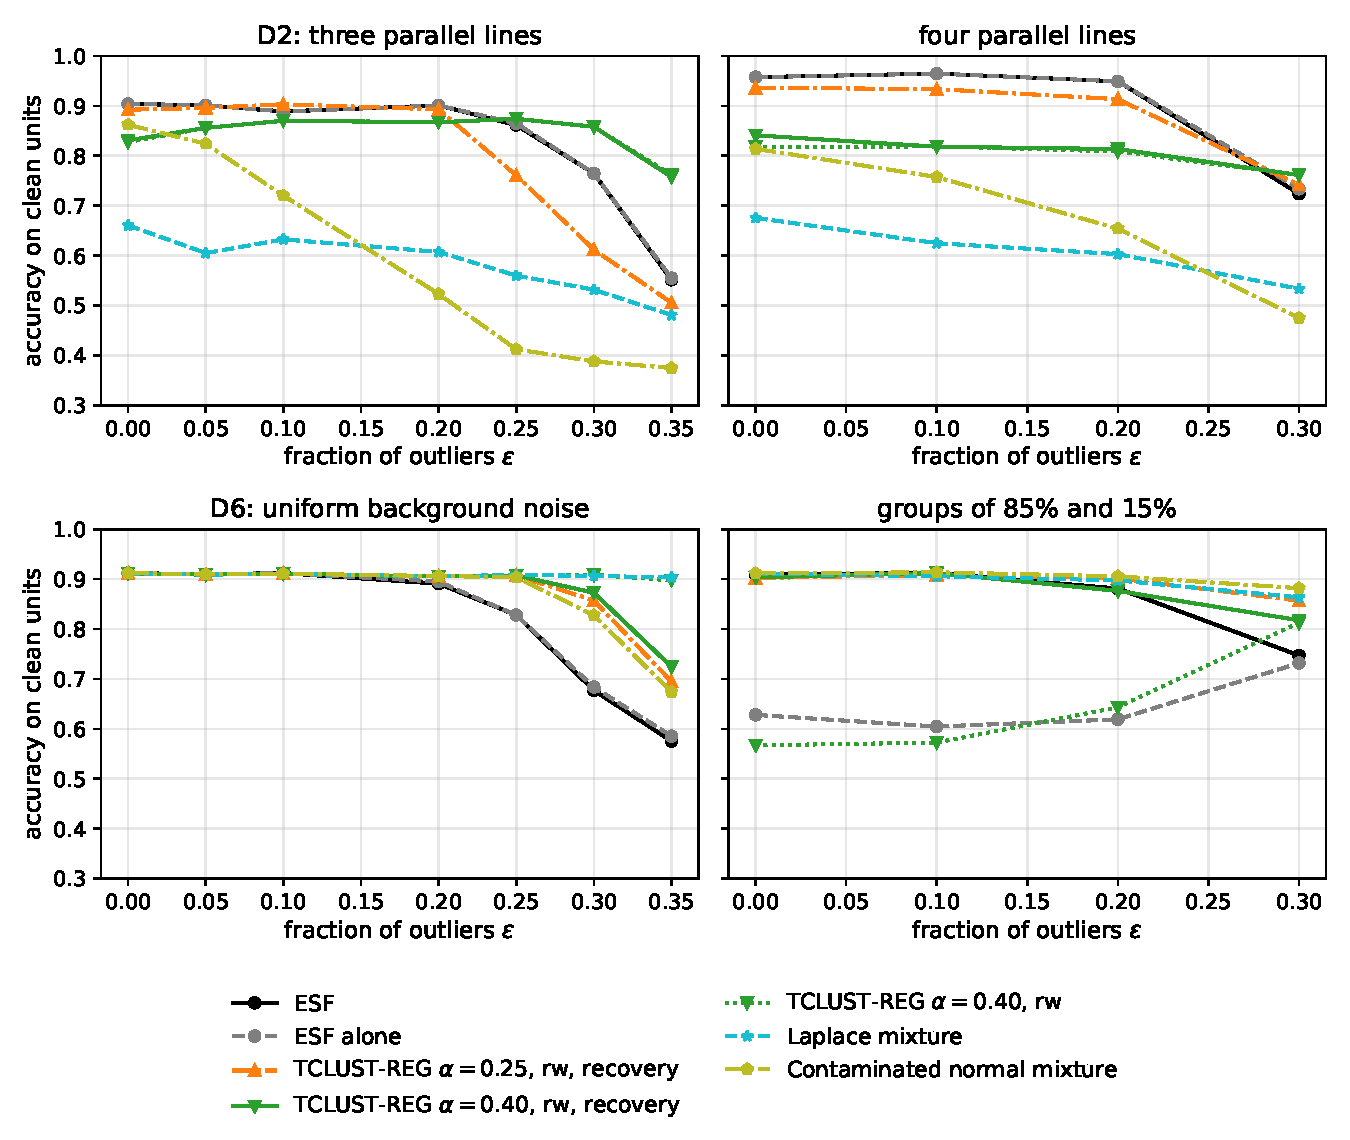
\includegraphics[width=0.9\textwidth]{figures/curves2.pdf}
\caption{Mean accuracy on clean units against the fraction of outliers in four designs. D2 and D6:
first part ($\varepsilon\le0.20$, $50$ data sets each) and second part ($\varepsilon\ge0.25$, $100$
data sets each, new data); four groups and groups of $85\%$ and $15\%$: third part ($50$ data sets
each), which was run at $\varepsilon\le0.30$ only. TCLUST-REG with $1000$ starts; rw: reweighted
by our rule; recovery: followed by the recovery step.}
\label{fig:curves}
\end{figure}

The level $0.40$ is the more robust choice from $25\%$ of outliers. With reweighting and the
recovery step it is ahead of ESF by more than $0.03$ in $13$ of the $34$ cells and never behind
by as much (Table~\ref{tab:level}; Figure~\ref{fig:curves}). ESF breaks down in four
situations. With uniform background noise (D6) it falls to $0.83$ at $\varepsilon=0.25$ and
$0.58$ at $0.35$, while TCLUST-REG at level $0.40$ with reweighting and the Laplace mixture stay
at $0.90$, and the recovery step, applied after TCLUST-REG, lowers this to $0.72$
(Section~\ref{sec:gate2}). With three groups (D2) it falls to $0.76$ at $\varepsilon=0.30$ and
$0.55$ at $0.35$, against $0.86$ and $0.76$ for the level $0.40$, and with four groups at
$0.30$ they reach $0.72$ and $0.76$. With high-leverage outliers (D5) it falls to $0.64$ at
$\varepsilon=0.25$ and about $0.53$ beyond, where no method is reliable, the best of
Supplement Table~S11 being the trimmed cluster-weighted model at level $0.40$ ($0.83$ at
$\varepsilon=0.25$, $0.70$ at $0.35$). With a small group or clustered outliers at $30\%$ it reaches $0.75$ and $0.55$,
against $0.82$ to $0.87$ and $0.70$ for the level $0.40$. In D1, D4, D7 and D8 it holds up to
$35\%$ of outliers. The Laplace mixture is the strongest method without a level at high
contamination, at $0.90$ or more up to $\varepsilon=0.35$ in D1, D3, D4, D6, D7 and D8, but
it fails with three and four groups already without outliers ($0.66$ and $0.68$) and with
clustered outliers.

\subsection{Covariate screen, other measures, further checks and cost}
\label{sec:measures}

\paragraph{The covariate screen.} It is what makes ESF robust to high-leverage points.
Without it (Supplement, Tables~S37 and~S38) the first step breaks down in D5 at
$\varepsilon=0.20$, as least squares does; outside D5 the two versions differ by at most $0.03$ up to
$\varepsilon=0.20$ in the first two parts, and from $\varepsilon=0.25$ on the screen gains up to $0.13$ and costs at
most $0.02$. The coefficient error (Supplement, Table~S19) tells the same story as the
accuracy: up to $\varepsilon=0.20$ the median error of ESF is at most $0.24$ in every design
D1 to D8, and it exceeds $1$ only where its accuracy has broken down.

\paragraph{The flagged fraction.} Where ESF works, its mean flagged fraction $\hat\alpha$
(Supplement, Table~S31) lies within about three percentage points of $\varepsilon$, and the
flagged set contains at least $89\%$ of the outliers and about $3\%$ of the clean units or
fewer (Supplement, Table~S16); where ESF breaks down it falls well below $\varepsilon$, because
the outliers are absorbed into a fitted line, which is the warning sign. After TCLUST-REG at
either conservative level, reweighting and the recovery step, the flagged fraction is as
close to $\varepsilon$ as that of ESF (mean absolute deviation over the $89$ cells with
$\varepsilon\le0.20$: $0.016$ and $0.017$ at the two levels, against $0.018$).

\paragraph{Further checks.} Supplement Section~S6 and Table~S39 report TCLUST-REG with equal
scales, with adaptive second-level trimming in the covariates and with a level chosen from its
monitoring path, the mixture of $t$ regressions \citep{yao2014robust}, robust linear grouping \citep{garciaescudero2009robust}, the incremental
reweighting of \citet{dotto2018reweighting}, two changes to our own constants, and the
mixtures with more starts (Tables~S21 and~S27). None gave a TCLUST-REG without a level or did
better than the pipelines above: the monitoring rules chose either a level below the
contamination or, nearly always, $0.40$, and the incremental reweighting fell below $0.85$ in
$22$ cells with $\varepsilon\le0.20$ after the recovery step, against four for the single
step.

\paragraph{Cost.} On one core ESF took a median of $0.08$ seconds per data set and about two
seconds with three covariates, most of it in the covariate screen; the times of the
competitors are in Supplement Table~S32.

\subsection{Sample size, groups, covariates and outliers}
\label{sec:further}

The third, descriptive part of the study ($2{,}300$ data sets, $50$ per cell) varied what the
first two held fixed: the sample size ($n=100$ and $n=1000$); the number of groups (four
parallel lines four noise scales apart, $n=400$, $m=16$); dependent covariates; moderate
outliers shifted by $4$ to $8$ noise scales, and outliers in a tight cloud; groups of $80\%$
and $20\%$ ($m=16$) and of $85\%$ and $15\%$ ($m=20$); and $t_3$ errors. Plan~5 added skewed
errors, groups of $70\%$ and $30\%$ with three covariates ($m=16$), and an error scale growing
fourfold over the design range (Supplement, Table~S25 and Section~S6). The sample size,
dependent covariates and moderate outliers change little: ESF stays within $0.014$ of the best
competitor chosen afterwards, except that with moderate outliers in D3 at $\varepsilon=0.30$ it
trails TCLUST-REG at level $0.25$ by $0.04$. Small groups are what the recovery step is for:
ESF alone reaches only $0.82$ without outliers and $0.73$ at $\varepsilon=0.20$ with groups of
$80\%$ and $20\%$, and between $0.60$ and $0.73$ with groups of $85\%$ and $15\%$, because its
best-scoring fit puts two nearly parallel lines on the large group and flags most of the small
one (Section~\ref{sec:algorithm}). With the recovery step it reaches $0.88$ to $0.91$ up to
$\varepsilon=0.20$, within $0.035$ of the best competitor, while at $\varepsilon=0.30$ the
first step flags more than a quarter of the units, the step rarely applies, and the accuracy
stays at $0.75$. Heavy-tailed, skewed and heteroscedastic errors leave the accuracy within
$0.006$ of the best competitor in every cell, but the flagged fraction then counts the tails
or the spread of the errors as well as the outliers: it exceeds the contamination by $6.5\%$
of the units with $t_3$ errors and no outliers and by $1$ to $6$ percentage points in Plan~5. Clustered outliers are the hard
case: at $\varepsilon=0.20$ ESF alone fits the cloud with one of its two lines and falls to
$0.70$; the recovery step repairs $11$ of the $27$ fits that fail in this way and raises the
mean to $0.78$, against $0.90$ for TCLUST-REG at a level above the contamination, and at
$\varepsilon=0.30$ no method of Table~\ref{tab:mainhigh} exceeds $0.72$.

\subsection{The recovery step: confirmation, sensitivity and repeated runs}
\label{sec:gate2}

The recovery step was developed on data generated with other seeds and frozen before Plan~3,
which applied it to the stored fits of ESF alone on the $6{,}400$ data sets the study then
held. All three criteria were met: in the six small-group cells with $\varepsilon\le0.20$ the
step raised the mean accuracy by $0.07$ to $0.31$ (at least $0.05$ was required), in no cell
with $\varepsilon\le0.20$ did it lower it by more than $0.004$ ($0.01$ was allowed), and the
comparison of Plan~1 was passed (Supplement, Table~S36). On the $600$ new data sets of Plan~4,
with two small-group designs not tried before (Supplement, Table~S41), the step raised the
accuracy by $0.09$ to $0.28$ in all $12$ cells, but with $20\%$ of outliers in the two new
designs ESF was $0.08$ and $0.09$ below TCLUST-REG at level $0.25$ with reweighting and the
recovery step ($0.91$ and $0.97$); in the other ten cells it was within $0.024$ of it.

\paragraph{Sensitivity and repeated runs.} Moving each constant of the recovery step one step
down and one step up (Supplement, Tables~S23 and~S44) changed no cell mean by more than about
$0.03$, except the limit on the flagged fraction (Section~\ref{sec:constants}). The noise range
$R$, $1.1$ times the range of the response, is set by the most extreme units, and a larger range
makes the uniform component less likely, so that a band of outliers passes more easily as a
group. With $R$ doubled, as if the most extreme unit lay twice as far out, the mean accuracy of
ESF up to $20\%$ of outliers moved from $0.914$ to $0.912$, but clustered outliers at
$\varepsilon=0.20$ lost $0.09$; with $R$ five times larger the losses reached $0.14$ with uniform
noise at $\varepsilon=0.20$, and after TCLUST-REG at level $0.40$ up to $0.29$ beyond $25\%$
(Supplement, Table~S48). Two ranges tied to the fitted scales, $20$ median scales and the range
of the unflagged units plus $10$ median scales, remove this dependence but make the uniform
component more likely everywhere and lose small groups: the mean accuracy of ESF up to $20\%$
fell to $0.891$ and $0.903$, with $12$ and $9$ cells below $0.85$ against two. The range of the
paper is the best of the three on these designs, at the price of a dependence on the most
extreme units. ESF depends on
its seed: in five runs with different seeds on each data set, the accuracies differed by more
than $0.05$ on $3.5\%$ of the data sets with up to $20\%$ of outliers and on $13\%$ of all
data sets, most of them where ESF breaks down (Supplement, Section~S6); this variation is of
the size of the thresholds of the plans, so the paired comparisons resolve differences of
about $0.03$ and no finer.

\paragraph{The recovery step after a trimming method.} After TCLUST-REG at level $0.40$ with
reweighting, the recovery step repairs the failures of the level with unequal groups up to
$\varepsilon=0.20$ (Section~\ref{sec:low}; Supplement, Table~S40) but not with three or four
groups, and it harms it materially once in the study (elsewhere by at most $0.016$):
with uniform noise at $30\%$ and $35\%$ it lowers the accuracy from $0.91$ to $0.87$ and from
$0.90$ to $0.72$, on $47$ of the $100$ data sets at $35\%$ by more than $0.05$, because a dense
and narrow band of uniform noise passes the peak test (Section~\ref{sec:recovery-theory}).
Moving each constant of the step did not prevent it (Supplement, Section~S5).
After the trimmed cluster-weighted model with reweighting (Supplement, Table~S46) the step did
the same: up to $\varepsilon=0.20$ it reduced the cells below $0.85$ from $39$ to $12$ at level
$0.25$ and from $66$ to $20$ at level $0.40$, and it lowered a cell mean by more than $0.02$
only with uniform noise at $30\%$ and $35\%$ (by up to $0.06$) and once with two parallel
lines at $30\%$ ($0.025$).
